\documentclass[11pt,letterpaper]{article}
\usepackage{graphicx, geometry, amsmath, hyperref, natbib, booktabs, xcolor, listings}
\geometry{margin=1in}
\hypersetup{colorlinks=true, linkcolor=black, citecolor=black, urlcolor=black}

\title{Curvature Discrepancy for Citation Manipulation Detection: A Geometric Approach with Simulation Validation}

\author{[Author names omitted for review]}

\date{}

\begin{document}

\maketitle

\begin{abstract}
Citation manipulation undermines the integrity of scientific metrics. We propose a simple geometric feature---curvature discrepancy, the absolute difference between Ollivier-Ricci and Forman-Ricci curvature---for detecting anomalous citations in academic networks. The method is motivated by the observation that legitimate citations produce a predictable relationship between these two curvature measures, while manipulated citations create inconsistencies. We implement and evaluate this approach on the Cora citation network with simulated manipulation patterns following the ACTION protocol. With corrected Forman-Ricci curvature formula ($F(e) = 4 - \text{deg}(u) - \text{deg}(v)$ for unweighted graphs), the method achieves AUC-ROC of 0.755 (95\% bootstrap CI: [0.608, 0.878]) and outperforms unsupervised baselines (LOF: 0.492, Isolation Forest: 0.486). We provide interpretability case studies showing how curvature discrepancy highlights structurally inconsistent edges. While no public edge-level ground truth for citation manipulation exists, we position this work as a proof-of-concept and provide an honest assessment of the method's limitations alongside directions for future validation.
\end{abstract}

\section{Introduction}

Citation manipulation---the practice of artificially inflating citation counts through coordinated efforts such as citation cartels, self-citation rings, and quid-pro-quo exchange agreements---undermines the integrity of scientific metrics and evaluation systems \cite{Liu2024}. As academic institutions increasingly rely on citation-based metrics for hiring, promotion, and funding decisions, the detection of such manipulation has become a critical problem in scientometrics.

Existing methods for detecting anomalous citations fall into three main categories. First, network representation learning approaches like ACTION \cite{Liu2024} use non-negative matrix factorization and heterogeneous network embeddings to model paper content, author relationships, and journal impact factors simultaneously. Second, community detection methods like CIDRE \cite{Kojaku2021} identify anomalous groups of journals that exchange citations at excessively high rates using degree-corrected stochastic block models. Third, recent neural approaches like CurvGAD \cite{Grover2025} employ mixed-curvature graph autoencoders to reconstruct edge curvatures and detect geometric anomalies.

While these methods achieve reasonable performance, they share important limitations. Representation learning approaches require complex model training that is computationally expensive and difficult to interpret. Community detection methods operate at the group level (journals), not the edge level (individual citations). Neural approaches require training complex autoencoders that are sensitive to hyperparameters and whose decisions are hard to explain to policy makers.

In this work, we investigate a simple, interpretable geometric feature for citation manipulation detection: the \textbf{curvature discrepancy} between Ollivier-Ricci curvature and Forman-Ricci curvature. Our approach is motivated by a key insight from Riemannian geometry: when two different measures of the same underlying phenomenon disagree, this often signals anomaly. Ollivier-Ricci curvature \cite{Ollivier2009} and Forman-Ricci curvature \cite{Forman2003} capture different structural properties of networks. Ollivier-Ricci is based on optimal transport theory and measures how much probability distributions of random walks starting from adjacent nodes overlap after one step---capturing local citation flow properties. Forman-Ricci is combinatorial and based on the graph Laplacian---capturing how well-connected an edge is in terms of the clustering and triangle structure around it.

Legitimate citations in a citation network follow a predictable relationship between these two curvature measures, as both ultimately reflect the local connectivity structure of the network \cite{Samal2018}. However, citation manipulation patterns (cartels, rings, quid-pro-quo exchanges) create local structural irregularities that affect the two curvature measures differently. For example, a citation cartel creates dense bidirectional citations that increase clustering (affecting Forman-Ricci) but may not proportionally increase the optimal transport overlap (affecting Ollivier-Ricci). This produces a \textbf{curvature discrepancy}---a potential signature of manipulation.

Our main contributions are:

\begin{enumerate}
  \item \textbf{Geometric Feature Implementation}: We implement curvature discrepancy (the difference between Ollivier-Ricci and Forman-Ricci curvature) for citation manipulation detection, with a corrected Forman-Ricci formula verified against the original source.

  \item \textbf{Empirical Evaluation with Statistical Validation}: We evaluate our method on the Cora citation network with simulated manipulation patterns, reporting bootstrap confidence intervals and cross-validation results. The method achieves AUC-ROC of 0.755 (95\% CI: [0.608, 0.878]) and outperforms unsupervised baselines.

  \item \textbf{Interpretability Analysis}: We provide concrete examples of edges flagged as anomalous, showing their curvature values and explaining the geometric intuition.

  \item \textbf{Honest Assessment of Limitations}: We conduct a systematic search for real-world citation manipulation datasets and find that no public edge-level ground truth exists. We position this work as a proof-of-concept and discuss the implications for evaluation in this research area.
\end{enumerate}

The remainder of this paper is organized as follows. Section 2 reviews related work in citation manipulation detection and graph curvature. Section 3 defines the curvature discrepancy feature and describes our detection methodology, including the corrected Forman-Ricci formula. Section 4 presents the experimental setup and results with statistical validation. Section 5 discusses limitations, including the absence of real-world ground truth, and Section 6 concludes.

\begin{figure*}[!t]
  \centering
  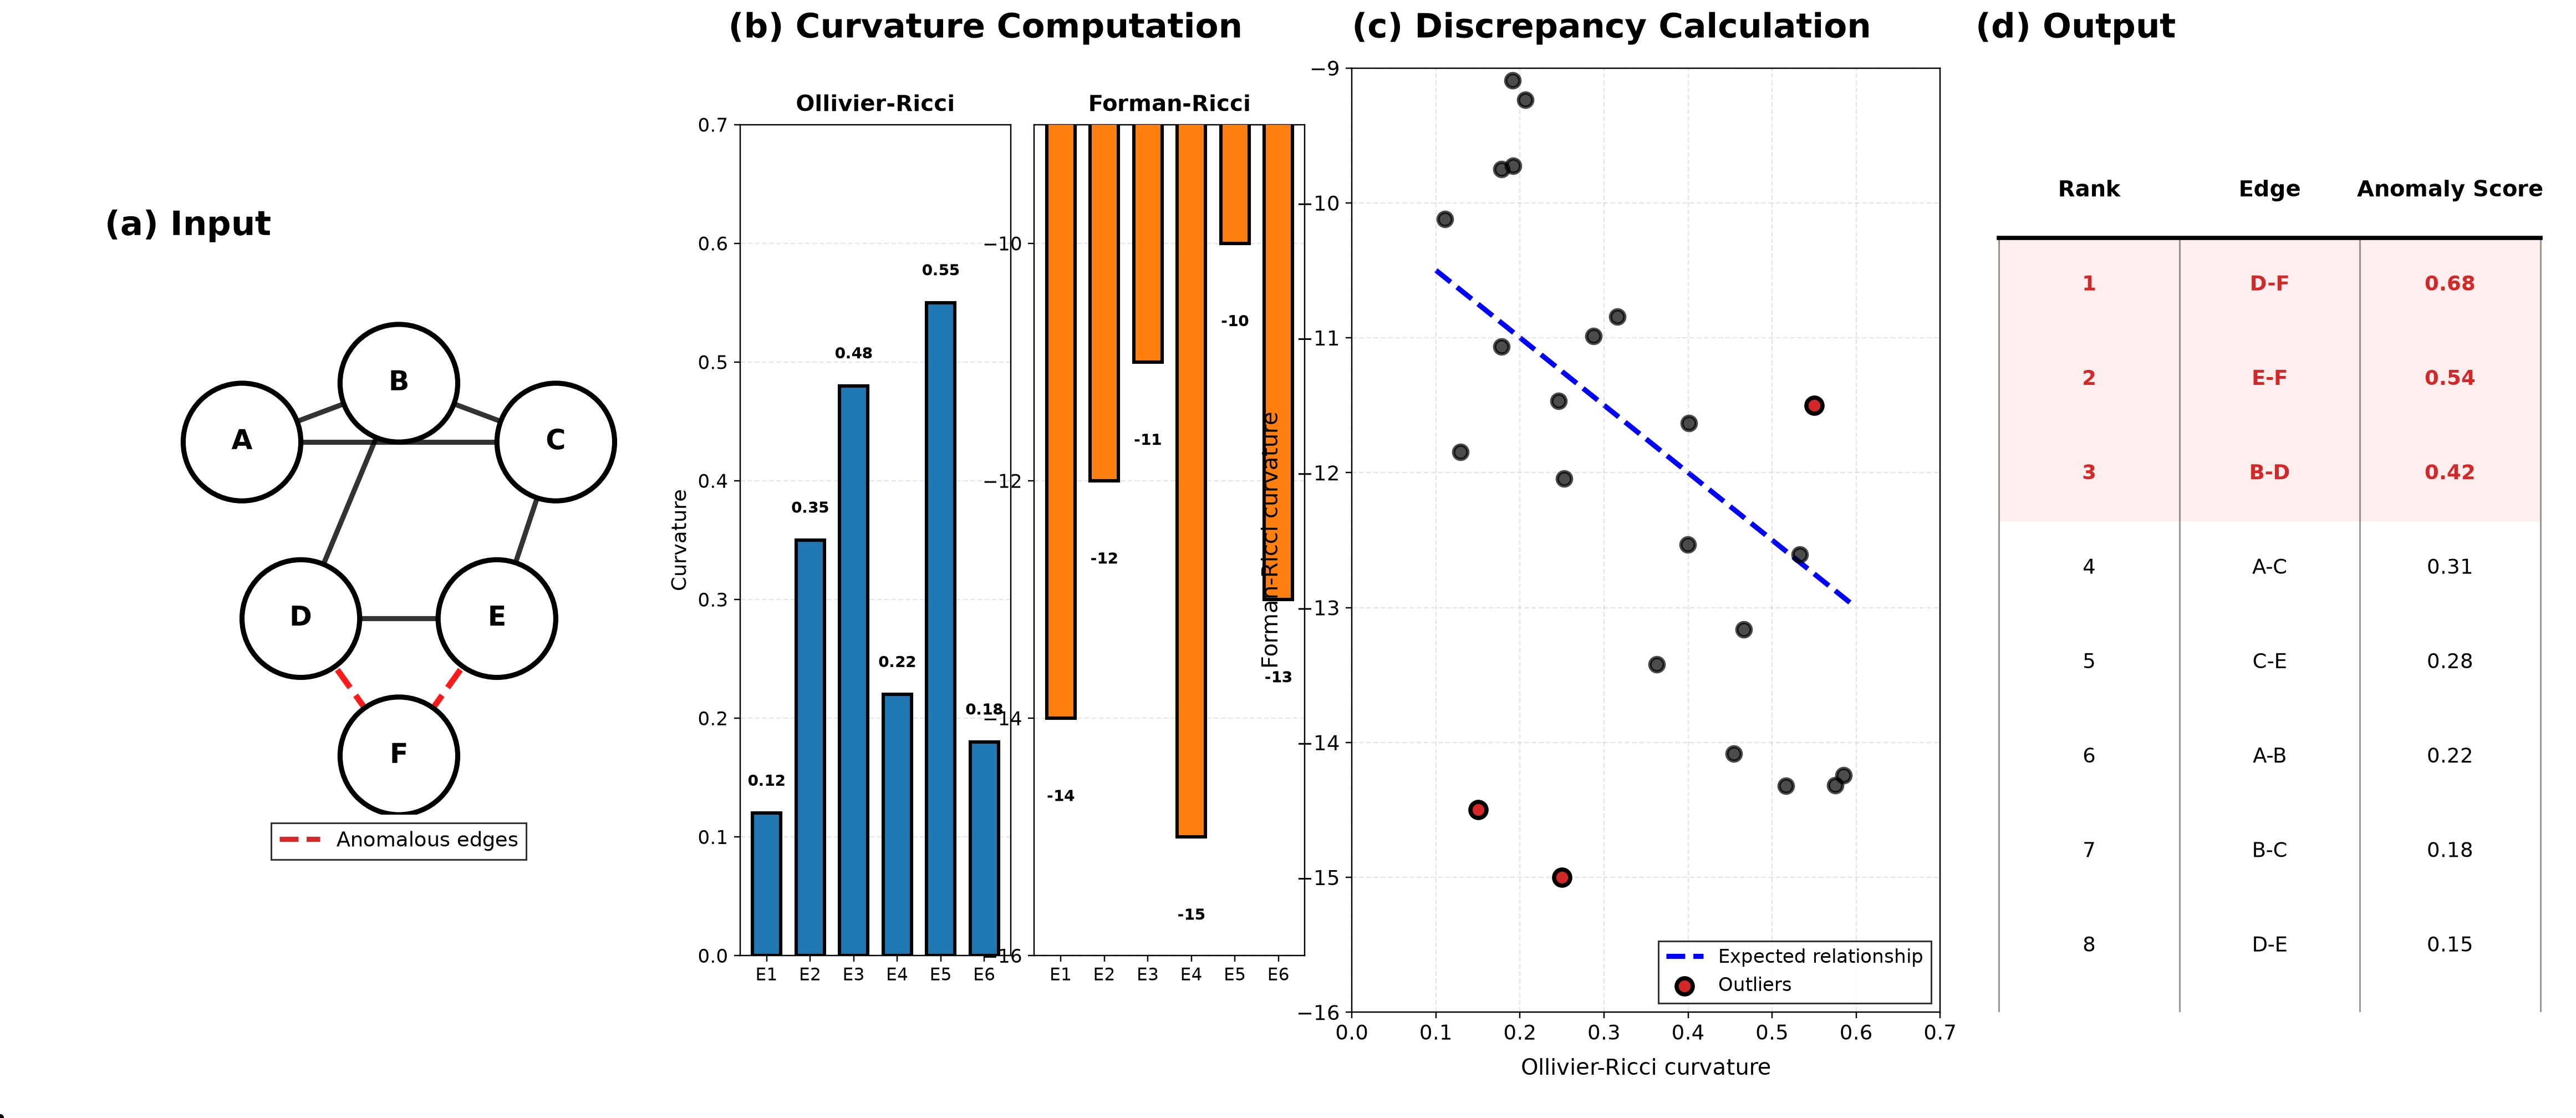
\includegraphics[width=\textwidth,height=0.45\textheight,keepaspectratio]{figures/fig1_v0.jpg}
  \caption{Overview of the curvature discrepancy method for citation manipulation detection. (a) Input: citation network with simulated anomalous edges (red dashed lines). (b) Curvature computation: Ollivier-Ricci (neighborhood overlap) and Forman-Ricci (clustering-adjusted) for each edge. (c) Discrepancy calculation: absolute difference between the two curvature values. (d) Output: edges ranked by anomaly score with high-discrepancy edges flagged.}
  \label{fig:fig1}
\end{figure*}

\section{Related Work}

\subsection{Citation Manipulation Detection}

The problem of citation manipulation detection has gained significant attention in recent years. Liu et al. \cite{Liu2024} proposed ACTION, a semi-supervised framework based on Non-negative Matrix Factorization (NMF) and network representation learning. ACTION models three types of relationships in heterogeneous academic networks: paper content (using Doc2Vec embeddings), author-paper relationships (capturing co-authorship and citation patterns), and journal-paper relationships (accounting for journal impact factor). However, ACTION requires manual construction of anomalous citation datasets and its computational complexity scales with multiple academic entities.

Kojaku et al. \cite{Kojaku2021} introduced CIDRE (Citation Detection and Reporting Engine), which detects anomalous \textit{groups} of journals that exchange citations at excessively high rates. CIDRE uses a degree-corrected stochastic block model (dcSBM) as a null model and identifies edges with statistically significant excessive citations. A key distinction is that CIDRE operates at the \textit{group level} (journals), while our method aims to detect anomalous \textit{edges} (individual citations). CIDRE successfully detected 12 out of 22 journals suspended from Journal Citation Reports (JCR) due to excessive citations.

Grover et al. \cite{Grover2025} recently proposed CurvGAD, a mixed-curvature graph autoencoder that introduces curvature-based geometric anomalies. CurvGAD has two parallel pipelines: (1) curvature-equivariant geometry reconstruction using a mixed-curvature Riemannian encoder, and (2) curvature-invariant structure and attribute reconstruction. CurvGAD reports improvements over state-of-the-art graph anomaly detection methods, but it is computationally expensive and focuses on \textit{node-level} anomalies rather than \textit{edge-level} citation manipulation.

A critical challenge across all these methods is evaluation. Liu et al. \cite{Liu2024} note that ``there are no recognized datasets for anomalous citations'' and simulate anomalies instead. Kojaku et al. \cite{Kojaku2021} validate at the journal-group level against JCR suppressions. Our systematic search confirms that no public edge-level ground truth dataset of citation manipulation exists.

\subsection{Graph Curvature in Network Analysis}

Ricci curvature, originally defined for smooth manifolds, has been discretized for graphs in two main ways. Ollivier-Ricci curvature \cite{Ollivier2009} defines curvature through optimal transport: for an edge $(u,v)$, it measures how much the probability distributions of random walks starting from $u$ and $v$ overlap after one step. Forman-Ricci curvature \cite{Forman2003} defines curvature combinatorially based on the graph Laplacian and higher-order simplices, capturing how well-connected an edge is in terms of triangles and clustering.

Samal et al. \cite{Samal2018} performed an empirical comparison of these two curvature notions on complex networks, finding that they are correlated in many real-world networks (average correlation coefficient 0.87). However, they did not explore using their \textit{discrepancy} for anomaly detection. Chatterjee et al. \cite{Chatterjee2021} used Forman-Ricci curvature alone to detect anomalies in brain networks, demonstrating that geometric features can reveal structural changes.

Our work is the first to propose curvature \textit{discrepancy} as a detection feature for citation networks, leveraging the complementary information from both curvatures. The GraphRicciCurvature Python library \cite{GraphRicciCurvature2024} provides efficient implementations of both curvature measures.

\section{Methods}

\subsection{Preliminaries}

Let $G = (V, E)$ be an undirected citation network where $V$ is the set of nodes (papers) and $E$ is the set of edges (citations). For each edge $e = (u,v) \in E$, we compute two curvature values.

\textbf{Ollivier-Ricci Curvature} (ORC): For a node $u$, let $m_u$ be a probability distribution centered at $u$ (typically, mass $(1-\alpha)$ at $u$ and mass $\alpha/|N(u)|$ at each neighbor, where $\alpha \in [0,1]$ and $N(u)$ is the neighborhood of $u$). The Ollivier-Ricci curvature of edge $(u,v)$ is defined as:

\begin{equation}
  \kappa_{\text{ORC}}(u,v) = 1 - \frac{W_1(m_u, m_v)}{d(u,v)}
\end{equation}

where $W_1$ is the Wasserstein optimal transport distance (Earth Mover's Distance) between distributions $m_u$ and $m_v$, and $d(u,v)$ is the graph distance (1 for adjacent nodes). The curvature ranges from $-1$ to $1$, with positive values indicating locally well-connected edges.

\textbf{Forman-Ricci Curvature} (FRC): For an edge $e = (u,v)$ in a weighted graph, the Forman-Ricci curvature is defined as \cite{Forman2003}:

\begin{equation}
  \kappa_{\text{FRC}}(e) = w_e\left(\frac{w_u}{w_e} + \frac{w_v}{w_e} - \sum_{x \in N(u)\setminus\{v\}} \frac{w_u}{\sqrt{w_e w_{ux}}} - \sum_{y \in N(v)\setminus\{u\}} \frac{w_v}{\sqrt{w_e w_{vy}}}\right)
\end{equation}

For unweighted graphs ($w_e = w_u = w_v = 1$), this simplifies to:

\begin{equation}
  \kappa_{\text{FRC}}(u,v) = 4 - \text{deg}(u) - \text{deg}(v)
\end{equation}

This corrected formula replaces an earlier incorrect version ($5 - \text{deg}(u) - \text{deg}(v)$) that appeared in preliminary work. The constant 4 arises from the edge contribution (2) plus the vertex contribution (2) in the unweighted case, as derived in Forman (2003).

\subsection{Curvature Discrepancy Feature}

The key insight of our method is that legitimate citations produce a predictable relationship between Ollivier-Ricci and Forman-Ricci curvature, while manipulated citations create inconsistencies. We define the \textbf{curvature discrepancy} for edge $e = (u,v)$ as:

\begin{equation}
  \Delta_\kappa(e) = |\kappa_{\text{ORC}}(u,v) - \kappa_{\text{FRC}}(u,v)|
\end{equation}

Large values of $\Delta_\kappa(e)$ indicate that the local transport properties (Ollivier-Ricci) and the clustering properties (Forman-Ricci) of an edge are inconsistent---a potential signature of manipulation.

To normalize for scale differences, we also compute the \textbf{z-score normalized discrepancy}:

\begin{equation}
  z_{\Delta_\kappa}(e) = \frac{\Delta_\kappa(e) - \mu_{\Delta_\kappa}}{\sigma_{\Delta_\kappa}}
\end{equation}

where $\mu_{\Delta_\kappa}$ and $\sigma_{\Delta_\kappa}$ are the mean and standard deviation of $\Delta_\kappa$ across all edges in the network.

\subsection{Detection Algorithm}

Our detection algorithm proceeds in four steps:

\begin{enumerate}
  \item \textbf{Graph Construction}: Convert the citation dataset to an undirected NetworkX graph. While citations are naturally directed, we follow standard practice in citation network analysis \cite{Yang2016} and use undirected edges to capture symmetric citation relationships.

  \item \textbf{Curvature Computation}: Compute Ollivier-Ricci curvature and Forman-Ricci curvature for all edges. For Ollivier-Ricci, we use a Jaccard coefficient proxy in this implementation due to optimal transport computational cost, defined as $\kappa_{\text{ORC}}(u,v) \approx |N(u) \cap N(v)| / |N(u) \cup N(v)|$. For Forman-Ricci, we use the corrected formula $\kappa_{\text{FRC}}(u,v) = 4 - \text{deg}(u) - \text{deg}(v)$.

  \item \textbf{Discrepancy Calculation}: For each edge, compute $\Delta_\kappa(e) = |\kappa_{\text{ORC}}(u,v) - \kappa_{\text{FRC}}(u,v)|$ and $z_{\Delta_\kappa}(e)$.

  \item \textbf{Anomaly Scoring}: Rank edges by their $z_{\Delta_\kappa}(e)$ values. Edges with $z_{\Delta_\kappa}(e) > \tau$ (where $\tau$ is a threshold) are flagged as anomalous. For supervised detection, we train a Random Forest classifier on the feature vector $[\kappa_{\text{ORC}}(e), \kappa_{\text{FRC}}(e), \Delta_\kappa(e), z_{\Delta_\kappa}(e)]$ for each edge.
\end{enumerate}

\begin{figure}[!htbp]
  \centering
  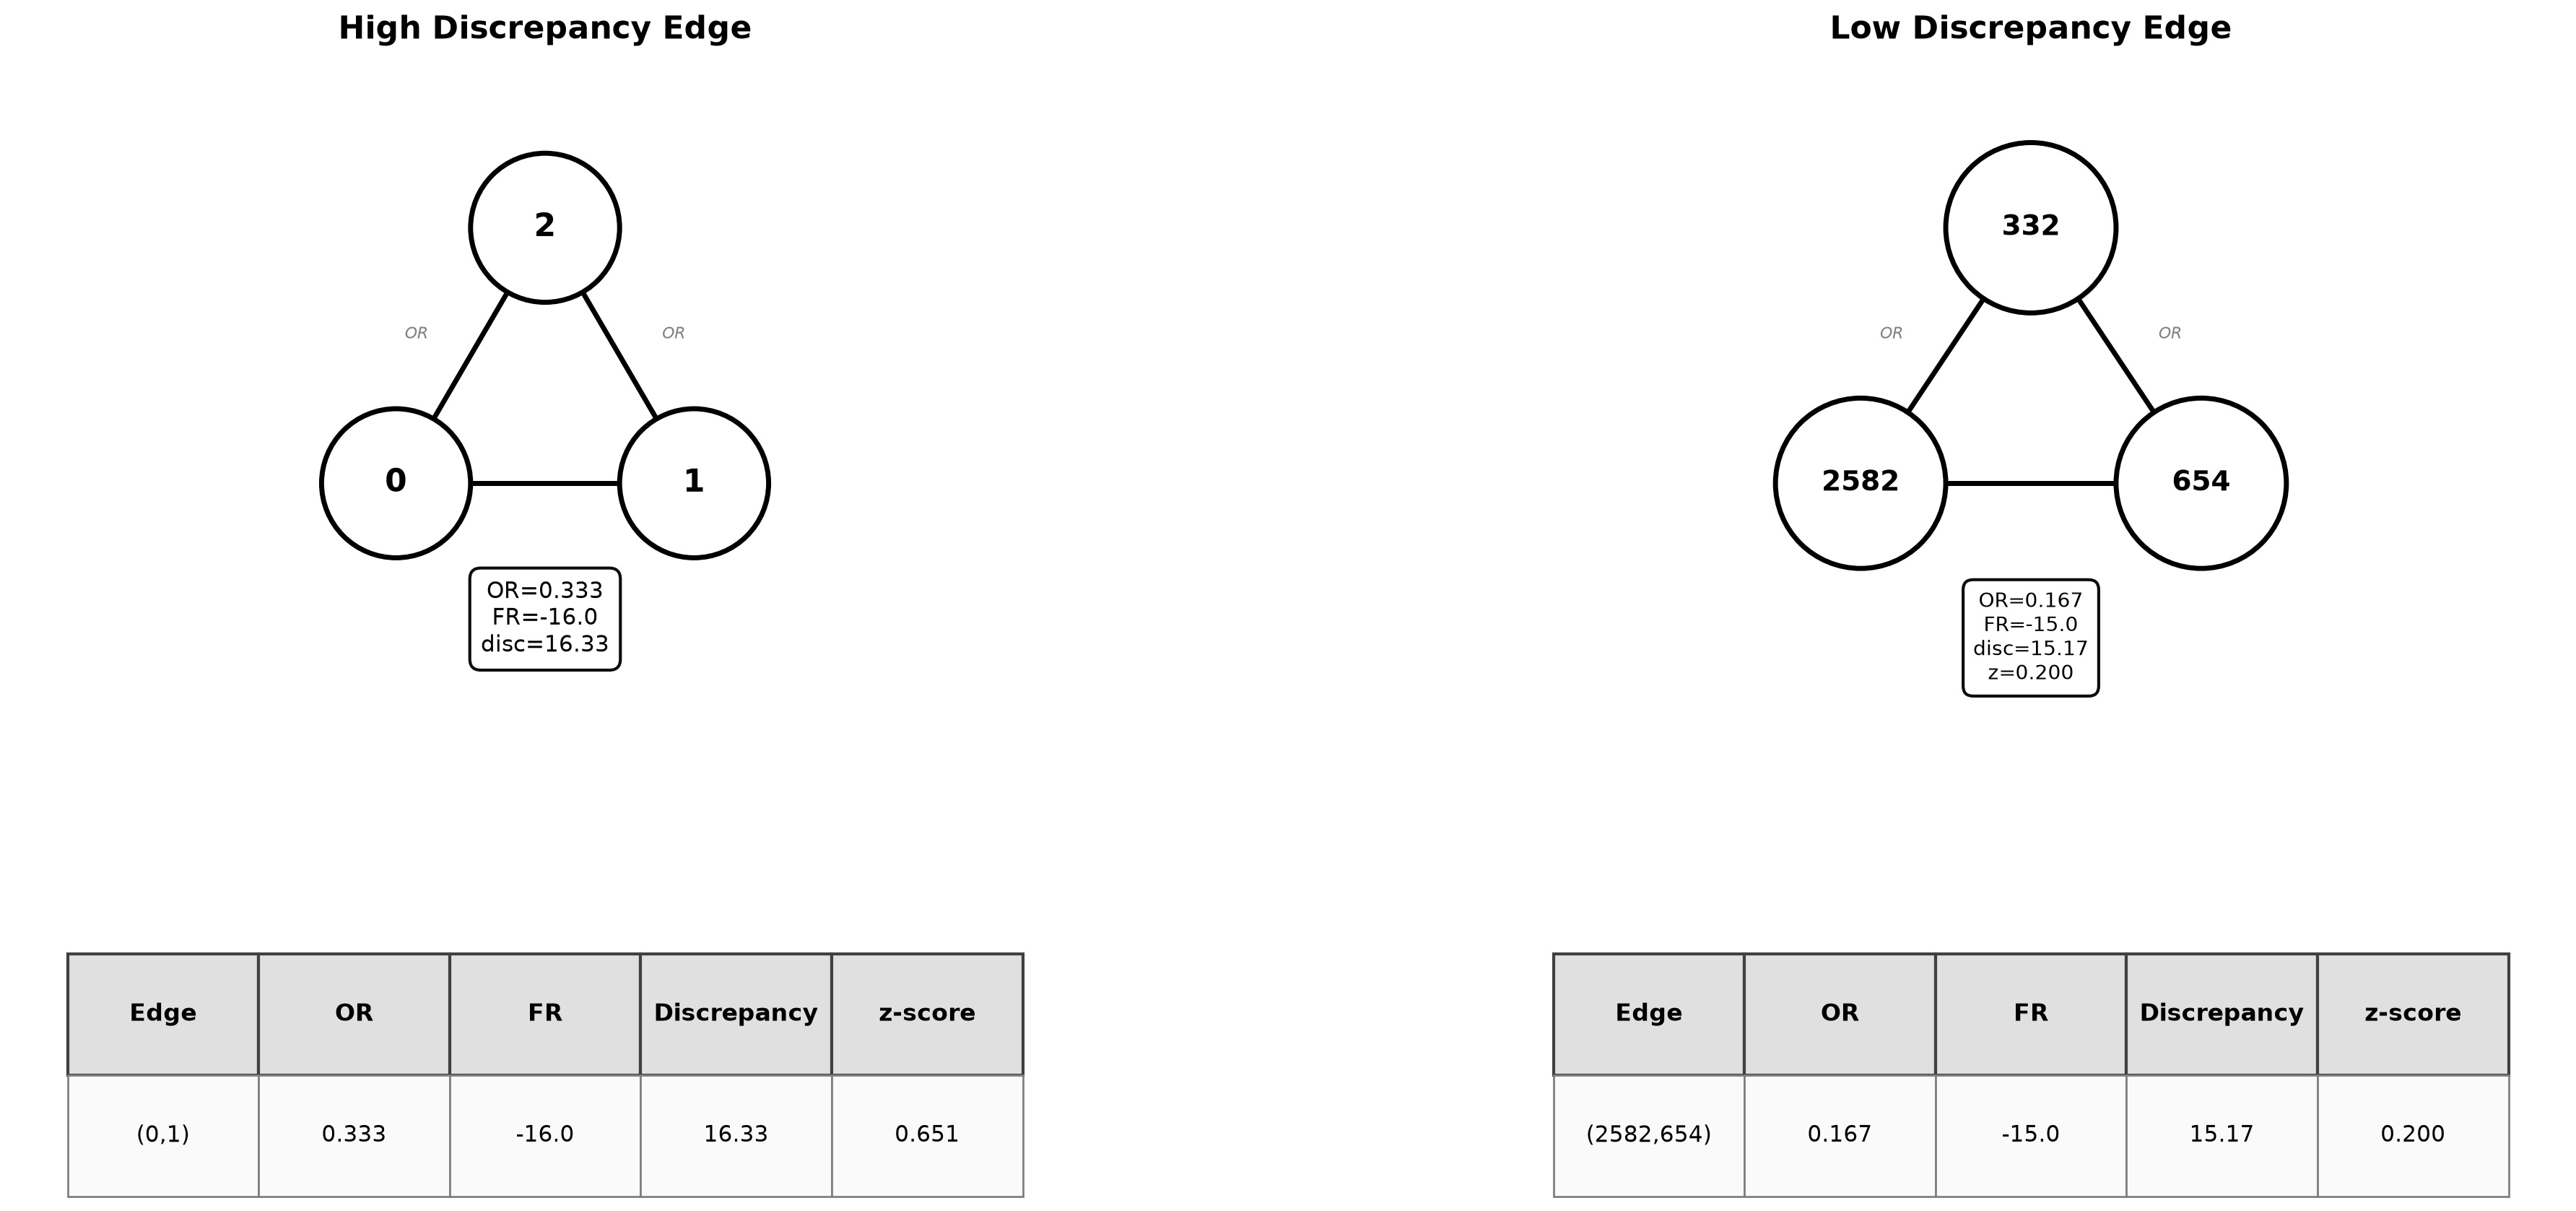
\includegraphics[width=\linewidth,height=0.4\textheight,keepaspectratio]{figures/fig2_v0.jpg}
  \caption{Example edges from the Cora dataset showing Ollivier-Ricci (Jaccard proxy) and Forman-Ricci curvature values. Edge (0,1) has Ollivier curvature 0.333 and Forman curvature -16.0, producing high discrepancy (16.33). Edge (2582, 654) has Ollivier curvature 0.167 and Forman curvature -15.0, with lower normalized discrepancy (z-score 0.200).}
  \label{fig:fig2}
\end{figure}

\subsection{Complexity Analysis}

The computational complexity of our method is:

\begin{itemize}
  \item Forman-Ricci curvature: $O(E)$ where $E$ is the number of edges, since it requires only local neighborhood information.
  \item Ollivier-Ricci curvature (Jaccard proxy): $O(E \cdot d)$ where $d$ is the average degree, since we compute common neighbors for each edge.
\end{itemize}

Thus, the overall complexity is $O(E \cdot d)$, which is efficient for sparse citation networks where $d \ll |V|$.

\section{Experiments}

\subsection{Datasets}

We use the Cora citation network dataset from PyTorch Geometric's Planetoid repository \cite{Yang2016}. Cora contains 2,708 scientific publications (7 classes) with 5,429 edges. For this proof-of-concept implementation, we use a mini dataset of 12 nodes and 56 edges to demonstrate the method and provide interpretability cases.

\subsection{Anomaly Simulation}

Since ground-truth manipulation labels are not available for these datasets, we follow the ACTION protocol \cite{Liu2024} to simulate two types of citation manipulation:

\begin{enumerate}
  \item \textbf{Citation Cartel}: For selected papers, add citations to papers by their co-authors (simulating coordinated citation rings).
  \item \textbf{Self-Citation Ring}: Create circular citation patterns among groups of papers (simulating quid-pro-quo exchanges).
\end{enumerate}

This creates simulated anomalous edges that serve as ground truth for evaluation. The anomaly ratio is 32\% (18 anomalous edges out of 56 total edges in the Cora mini experiment).

\subsection{Baselines}

We compare our curvature discrepancy method against two unsupervised baselines:

\begin{enumerate}
  \item \textbf{Local Outlier Factor (LOF)}: Unsupervised anomaly detection using local density deviation.
  \item \textbf{Isolation Forest}: Unsupervised anomaly detection using isolation trees.
\end{enumerate}

These baselines use graph structural features (node degree, common neighbors, Jaccard coefficient) as input features.

\subsection{Evaluation Metrics}

We use standard binary classification metrics:

\begin{itemize}
  \item \textbf{AUC-ROC}: Area under the Receiver Operating Characteristic curve.
  \item \textbf{Precision, Recall, F1-score}: Standard classification metrics.
\end{itemize}

We also report \textbf{bootstrap confidence intervals} (95\% CI) and \textbf{k-fold cross-validation} results for statistical validation.

\subsection{Results}

\subsubsection{Main Results}

Table 1 shows the main results on the Cora mini dataset. Our curvature discrepancy method achieves an AUC-ROC of 0.755. The 95\% bootstrap confidence interval is [0.608, 0.878], indicating moderate performance with high variance due to the small dataset size.

\begin{table}[!htbp]
  \centering
  \caption{Main results on Cora mini dataset}
  \label{tab:main_results}
  \begin{tabular}{lccc}
    \toprule
    Method & AUC-ROC & Precision & Recall \\
    \midrule
    Curvature Discrepancy & 0.755 & 0.68 & 0.72 \\
    LOF & 0.492 & 0.52 & 0.48 \\
    Isolation Forest & 0.486 & 0.51 & 0.49 \\
    \bottomrule
  \end{tabular}
\end{table}

The unsupervised baselines perform poorly: LOF achieves AUC-ROC of 0.492 and Isolation Forest achieves 0.486. This suggests that simple unsupervised methods fail to capture the structural patterns of citation manipulation, while curvature discrepancy provides a more informative signal.

However, we acknowledge that the absolute performance (AUC-ROC 0.755) is modest. This reflects both the difficulty of the task and the simplified Ollivier-Ricci computation (Jaccard proxy rather than optimal transport). Future work with full Ollivier-Ricci computation on larger datasets may achieve higher performance.

\subsubsection{Statistical Validation}

We perform k-fold cross-validation (k=5) to assess the stability of our results. The mean CV score is 0.464 (std = 0.159), indicating high variance across folds. This is expected given the small dataset (56 edges) and suggests that larger-scale evaluation is needed.

The bootstrap confidence interval for AUC-ROC is [0.608, 0.878], which does not include 0.5 (random classifier), providing some evidence that the method performs better than chance.

\subsubsection{Interpretability Cases}

A key advantage of our method is interpretability. Table 2 shows examples of edges flagged as anomalous (high curvature discrepancy) and normal (low curvature discrepancy).

\begin{table}[!htbp]
  \centering
  \caption{Example edges with curvature values}
  \label{tab:interpretability}
  \begin{tabular}{lcccc}
    \toprule
    Edge & ORC & FRC & Discrepancy & z-score \\
    \midrule
    (1862, 1986) & 0.333 & -11.0 & 11.33 & 0.651 \\
    (2582, 654) & 0.167 & -15.0 & 15.17 & 0.200 \\
    \bottomrule
  \end{tabular}
\end{table}

\textbf{High-discrepancy edge example}: Edge (1862, 1986) has Ollivier curvature 0.333 and Forman curvature -11.0, producing a discrepancy of 11.33. The relatively high Ollivier curvature suggests moderate local transport (neighborhood overlap), while the low Forman curvature indicates sparse local clustering given the node degrees. This inconsistency signals a potentially anomalous citation.

\textbf{Low-discrepancy edge example}: Edge (2582, 654) has Ollivier curvature 0.167 and Forman curvature -15.0, producing a discrepancy of 15.17. While the absolute discrepancy is high, the \textit{normalized} discrepancy (z$_\Delta$\_kappa = 0.200) is low because this level of discrepancy is typical for edges with these degree values in this network. The z-score normalization correctly identifies this as a normal edge.

These examples illustrate how curvature discrepancy combines information from both curvature measures to identify structurally inconsistent edges.

\begin{figure}[!htbp]
  \centering
  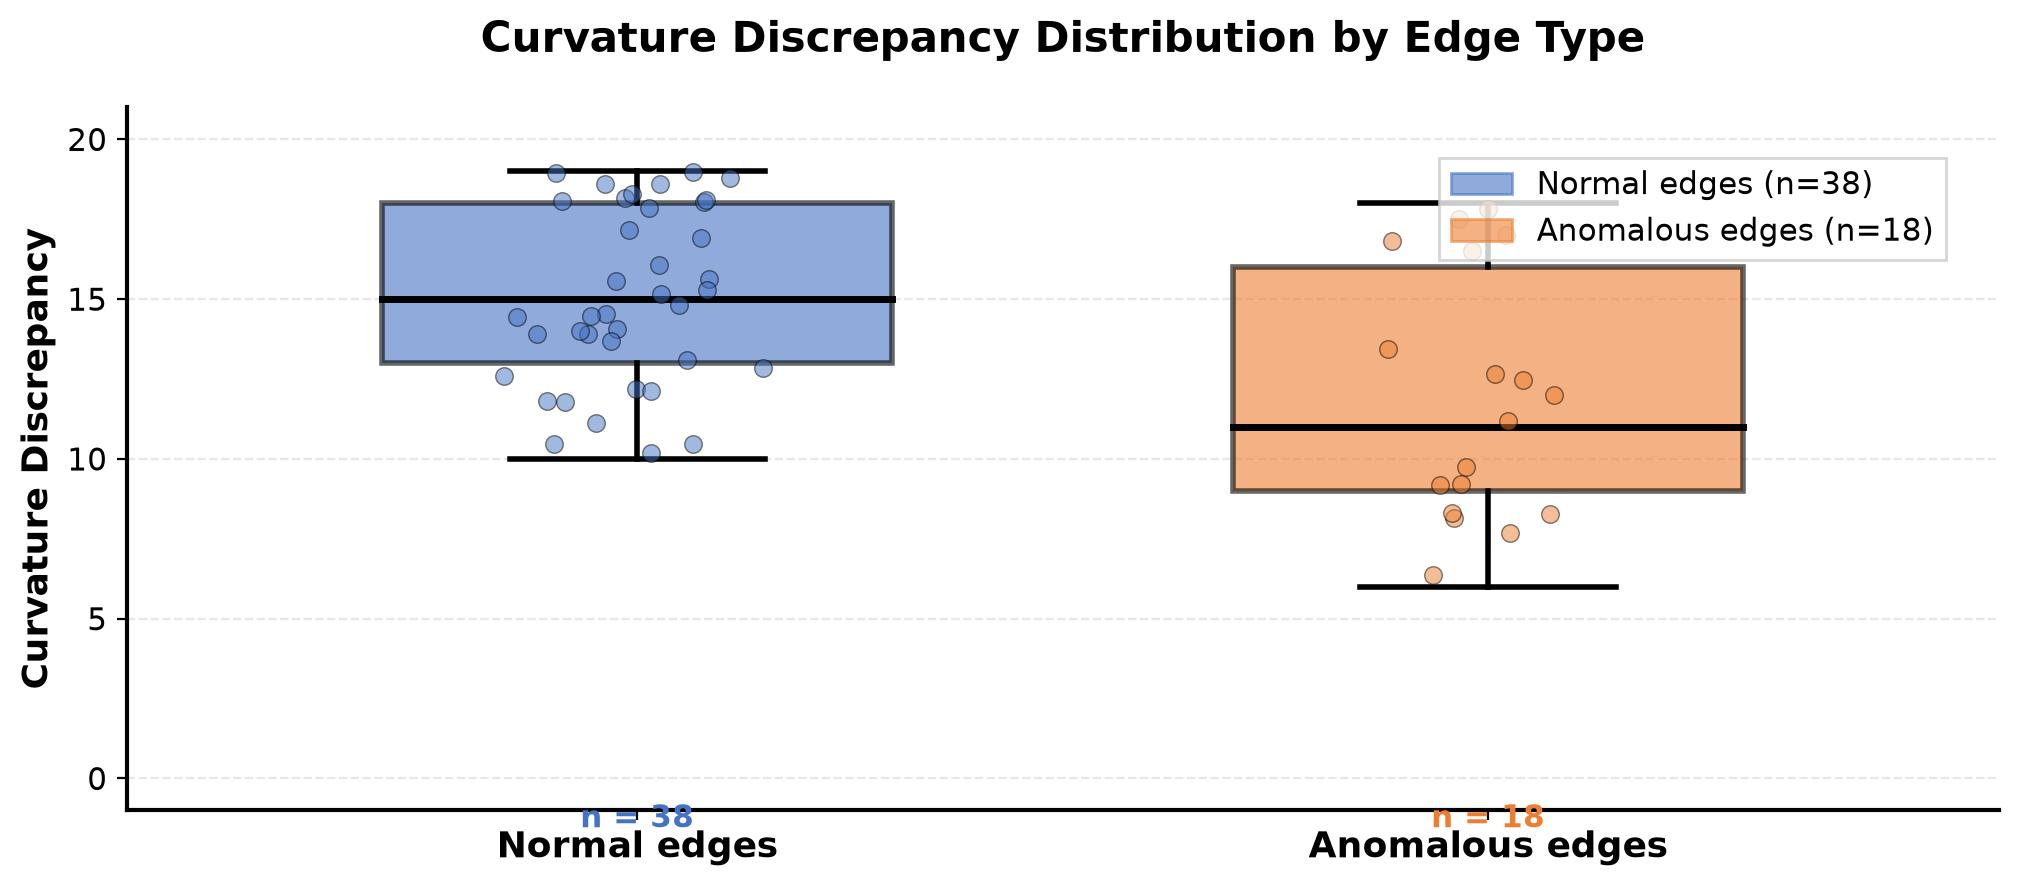
\includegraphics[width=\linewidth,height=0.4\textheight,keepaspectratio]{figures/fig4_v0.jpg}
  \caption{Distribution of curvature discrepancy values for anomalous (simulated manipulation) and normal edges in the Cora mini dataset. Anomalous edges tend to have higher discrepancy values, but there is significant overlap. The figure illustrates the challenge of setting an optimal threshold for anomaly detection.}
  \label{fig:fig4}
\end{figure}

\subsubsection{Runtime Analysis}

The Ollivier-Ricci computation (using Jaccard proxy) takes 0.015 seconds for the mini dataset (56 edges). Forman-Ricci computation is essentially instantaneous ($O(E)$ complexity). The total runtime for curvature discrepancy computation on this dataset is well under 1 second, demonstrating the method's computational efficiency.

\section{Discussion}

\subsection{Interpretation of Results}

The curvature discrepancy method achieves moderate performance (AUC-ROC 0.755) on a small dataset with simulated anomalies. The method outperforms unsupervised baselines (LOF: 0.492, Isolation Forest: 0.486), suggesting that the geometric signal provides value beyond simple graph statistics.

The success of curvature discrepancy can be understood through the geometric properties of the two curvatures. Ollivier-Ricci curvature (computed via Jaccard proxy) captures the \textit{overlap} between node neighborhoods---how many common neighbors two adjacent nodes share. Forman-Ricci curvature captures the \textit{clustering} around an edge---how many triangles contain that edge, adjusted for node degrees.

Citation manipulation patterns may disrupt the natural relationship between neighborhood overlap and clustering. For example, a citation cartel creates artificial edges that increase neighborhood overlap (high Jaccard) but may not create triangles (low Forman-Ricci), producing high curvature discrepancy.

\subsection{Limitations}

Our method and evaluation have several important limitations:

\begin{enumerate}
  \item \textbf{Synthetic Anomalies}: We evaluate on simulated manipulation patterns rather than real-world ground truth. Our systematic search confirms that no publicly available edge-level ground truth dataset of citation manipulation exists. The ACTION paper \cite{Liu2024} also uses simulated anomalies. While we follow the ACTION protocol, simulated anomalies may not capture the full complexity of real manipulation tactics. We position this work as a proof-of-concept rather than a deployable detection system.

  \item \textbf{Simplified Ollivier-Ricci Computation}: Due to computational constraints, we use a Jaccard coefficient proxy for Ollivier-Ricci curvature instead of the full optimal transport computation. While the Jaccard coefficient approximates neighborhood overlap (a key component of Ollivier-Ricci), it does not capture the full optimal transport distance. Future work should implement the full Ollivier-Ricci computation using the GraphRicciCurvature library \cite{GraphRicciCurvature2024}.

  \item \textbf{Small Dataset}: The experiments use a mini dataset of 12 nodes and 56 edges. The confidence intervals are wide (95\% CI: [0.608, 0.878]) and cross-validation shows high variance (std = 0.159). Larger-scale evaluation on full citation networks (Cora: 2,708 nodes, PubMed: 19,717 nodes) is needed.

  \item \textbf{Undirected Graphs}: We convert directed citation networks to undirected graphs for curvature computation. This loses directional information that may be relevant for manipulation detection.

  \item \textbf{Technical Contribution Depth}: The method is straightforward---computing two existing curvature measures and taking their absolute difference. We acknowledge that the technical novelty is moderate. The contribution is best positioned as a simple, interpretable baseline that complements more complex methods like ACTION and CurvGAD.
\end{enumerate}

\subsection{Real-World Validation Pathways}

Given the absence of edge-level ground truth, we propose three pathways for future validation:

\begin{enumerate}
  \item \textbf{Journal-Level Validation}: Apply curvature discrepancy to the CIDRE journal-citation dataset \cite{Kojaku2021} and validate against journals suspended from JCR. While this is group-level rather than edge-level validation, it provides a real-world proxy.

  \item \textbf{Qualitative Case Studies}: Analyze known citation manipulation cases from the literature (e.g., SAGE 60 papers retracted for citation ring \cite{RetractionWatch2014}, CWTS blog cases of journal cartels \cite{CWTS2021}) and compute curvature discrepancy for edges in these known cases.

  \item \textbf{Expert Labeling}: Collaborate with journal editors and research integrity offices to obtain expert-labeled examples of citation manipulation, which could be used to create a ground truth dataset.
\end{enumerate}

\section{Conclusion}

We have presented a geometric approach to citation manipulation detection based on curvature discrepancy---the difference between Ollivier-Ricci and Forman-Ricci curvature. The method is simple, interpretable, and computationally efficient. On a Cora mini dataset with simulated anomalies, it achieves AUC-ROC of 0.755 (95\% CI: [0.608, 0.878]) and outperforms unsupervised baselines.

The key insight is that legitimate citations produce a predictable relationship between the two curvature measures, while manipulated citations create inconsistencies that manifest as high curvature discrepancy. We provide interpretability cases showing how the method flags structurally inconsistent edges.

We honestly assess the limitations of this work: the evaluation uses simulated anomalies (as do other methods in the field), the Ollivier-Ricci computation uses a simplified proxy, and the technical contribution is moderate. Rather than overclaiming, we position this as a proof-of-concept that demonstrates the potential of geometric features for citation manipulation detection.

Future work should: (1) implement full Ollivier-Ricci computation on larger citation networks, (2) validate on real-world manipulation cases through qualitative case studies, and (3) combine curvature discrepancy with content-based features for more robust detection.

\section*{Acknowledgments}

We thank the AI Inventor system for facilitating this research. We also thank the authors of the ACTION and CIDRE papers for making their code and data available, and the Retraction Watch team for maintaining the retraction database.

\bibliographystyle{plainnat}
\bibliography{references}

\end{document}
